
\documentclass{beamer}
\usepackage[utf8]{inputenc}

\usepackage[utf8]{inputenc}
\usepackage[T1]{fontenc}

\usepackage[english]{babel}
\usepackage{amsmath}
\usepackage{cleveref}
\usepackage{amssymb}
\usepackage{mathtools}

%%Numbers, expectation
\newcommand{\N}{\mathbb{N}}
\newcommand{\E}{\mathbb{E}}
\renewcommand{\P}{\mathbb{P}}
\newcommand{\Var}{\mathbb{V}}
\newcommand{\R}{\mathbb{R}}
\newcommand{\D}{\mathcal{D}}
\newcommand{\B}{\mathcal{B}}
\newcommand{\Dh}{\D_h}
\renewcommand{\phi}{\varphi}
\newcommand*\diff{\mathop{}\!\mathrm{d}} % integral

%% mathoperator
\DeclareMathOperator*{\argmax}{arg\,max}
\DeclareMathOperator*{\argmin}{arg\,min}
\DeclareMathOperator*{\dom}{dom}
\DeclareMathOperator*{\sign}{sign}
\DeclareMathOperator*{\diag}{diag}

\DeclareMathOperator*{\Cov}{Cov}
\DeclareMathOperator*{\Cor}{Corr}
\DeclareMathOperator*{\Id}{Id}

%proximal operator
\newcommand{\prox}[3][]{\operatorname{prox}^{#1}_{#2}\left(#3 \right)}

\usepackage{xcolor}

%% sort citations by increasing number
\usepackage[sort,nocompress]{cite}

\usepackage{graphicx}% http://ctan.org/pkg/graphicx
\graphicspath{{../figures/}{../../figures}{../../memes}} %Setting the graphicspath
\usepackage{caption,subcaption}

\usepackage{tikz}
\usepackage{pgfplots}
\usetikzlibrary{backgrounds}
\usetikzlibrary{intersections}
\usepgfplotslibrary{fillbetween}

% \usepackage[right]{showlabels}


%%
\theoremstyle{plain}
\newtheorem{prop}{Proposition}[section]
\newtheorem{algo}{Algorithm}[section]
\newtheorem{assumption}{Assumption}
\theoremstyle{remark}
\newtheorem{remark}{Remark}[section]

% cref
\crefname{assumption}{Assumption}{Assumptions}
\crefname{equation}{}{}

\usepackage{autonum}

\usepackage{bm} %% bold math symbols

\usepackage{bbm} %% for \mathbbm{1}


% algorithmic environment
\usepackage{algorithm}
\usepackage[noend]{algpseudocode}

% for some reason this was required on one void linux installation (but not the other)
\usepackage{sansmathaccent}
\pdfmapfile{+sansmathaccent.map}

\author{Axel Böhm}

% shows which section we're in
\usetheme{Darmstadt}

% page number
\setbeamertemplate{footline}[frame number]
\setbeamercolor{page number in head/foot}{fg=gray}


% display things like onslide or visible already before but grayed out
\setbeamercovered{transparent}

% set the itemize item symbol as a diamond
\setbeamertemplate{itemize item}{$\diamond$}
% set the itemize subitem symbol as a triangle
\setbeamertemplate{itemize subitem}{$\blacktriangleright$}

% set the enumerate item symbol as a roman numbers
\setbeamertemplate{enumerate item}{(\roman{enumi})}


% reference: https://indico.cern.ch/event/845380/attachments/1915103/3241592/Dvurechensky_lectures.pdf
% https://arxiv.org/abs/1803.00567

% Use this aswell
% https://www.math.ucdavis.edu/~qlxia/Research/monge.pdf

\title{Optimal Transport}
\date{\today}

\begin{document}
\maketitle
\frame{\tableofcontents[currentsection]}

\section{Monge Problem}%
\label{sec:}

\begin{frame}
  \frametitle{The Monge Problem (1781)}

  \begin{minipage}{0.5\textwidth}
    \begin{figure}[ht]
      \centering
      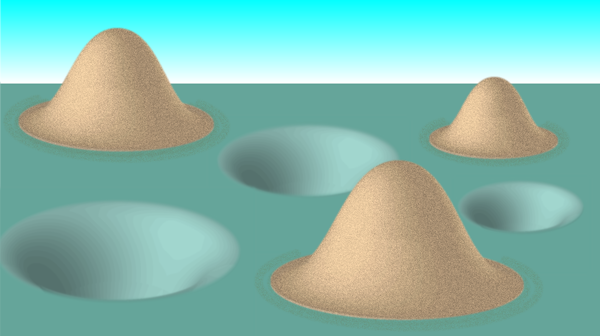
\includegraphics[width=\textwidth]{monge-sand.png}
      \caption{How to best move piles of sand to fill up holes of the same total volume?\label{fig:label} }
    \end{figure}
  \end{minipage}
  \hfill
  \begin{minipage}{0.45\textwidth}
    \begin{itemize}
      \item $X,Y$ are metric spaces
      \item $\B$ is a Borel $\sigma$-Algebra (open sets, countable union, \dots)
      \item $\mu$ is a probability measure
    \end{itemize}
  Given a cost $c: X\times Y \to \R_+$ find a \textbf{transport map} $T: X \to Y$ minimizing
  \begin{equation}
    M(\mu, \nu) = \inf_T \int_X c(x, Tx) \diff \mu(x)
  \end{equation}
  s.t.\ the \emph{mass} remains the same:
  \begin{equation}
    \mu(T^{-1}(B)) = \nu(B) \quad \forall B \in \B.
  \end{equation}
  \end{minipage}
\end{frame}

\begin{frame}
  \frametitle{Drawbacks of Monge formulation}
  \begin{block}{Example}
    $X=(x_1, \dots, x_m)$ and $Y=(y_1, \dots, y_n)$ and
    $\mu= \frac{1}{m}(\delta_{x_1}+ \dots + \delta_{x_m})$ and $\nu= \frac{1}{n}(\delta_{y_1}+ \dots + \delta_{y_m})$
  \end{block}
  \begin{minipage}{0.5\textwidth}
    \underline{If $m=n$}, then $c(\cdot, \cdot) = C \in \R^{m\times n}$ is just a (square) matrix and $T$ is a permutation $\sigma$
    \begin{equation}
      \begin{aligned}
        M(\mu, \nu) &= \min_T \frac{1}{n} \sum_{i} c(x_i, T(x_i)) \\
        &= \min_\sigma \frac{1}{n} \sum_{i} c(x_i, y_{\sigma(i)}) \\
        &= \min_\sigma \frac{1}{n} \sum_{i} C_{i, \sigma(i)} \\
      \end{aligned}
    \end{equation}
  \end{minipage}
  \hfill
  \begin{minipage}{0.4\textwidth}
    \underline{If $m \neq n$}, for example $\mu=\delta_{x_1}$ and $\nu= \frac12(\delta_{y_1}+ \delta_{y_2})$
    $\Rightarrow$ No $T$ exists.
    \vspace{3.5cm}
    \vfill
  \end{minipage}
\end{frame}

\begin{frame}
  \frametitle{Nonuniqueness of solutions}
  \begin{figure}[ht]
    \centering
    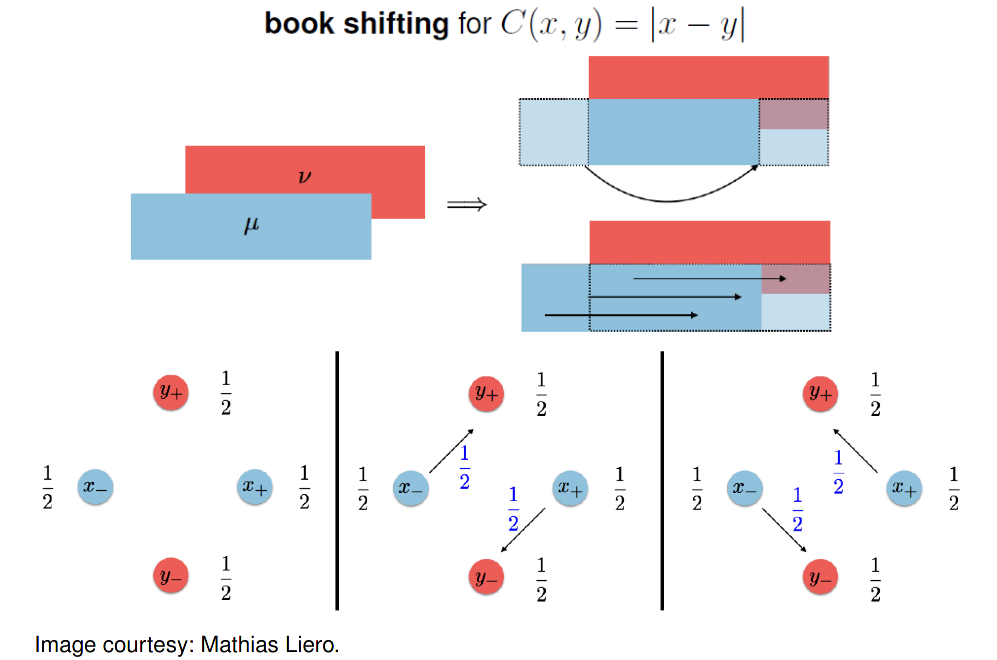
\includegraphics[scale=0.3]{book-shifting.png}
    \caption{\label{fig:label} }
  \end{figure}
\end{frame}

\section{Kantorovich formulation}%
\label{sec:}


\begin{frame}
  \frametitle{Kantorovich's relaxation (1940s)}
  % we allow for splitting the mass coming from one point (can be spread out)
  Before: \emph{Transport map}, $\forall x$ move all amount to some $y$.\\
  Now: \emph{Transport plan}, $\forall (x,y)$ how much to move from $x$ to $y$.

  \begin{block}{}
    Find $\gamma \in \P(X \times Y)$
    \begin{equation}
      \begin{aligned}
        K(\mu, \mu) &= \inf_{\gamma} \int_{X \times Y} c(x,y) \diff \gamma(x,y) \\
        \text{s.t.} & \gamma(A \times Y) = \mu(A) \\
                    & \gamma(X \times B) = \nu(B)
      \end{aligned}
    \end{equation}
    % Linear in \gamma
    for all $A \in \B(X)$ and $B \in \B(Y)$.
    Note: constraints say that $\mu$ and $\nu$ are the marginals of $\gamma$, i.e.\ $\gamma \in \Pi(\mu, \nu)$.
  \end{block}

\end{frame}

\begin{frame}
  \frametitle{Kantorovich's relaxation}
  Allows for many more settings.
  \begin{figure}[ht]
    \centering
    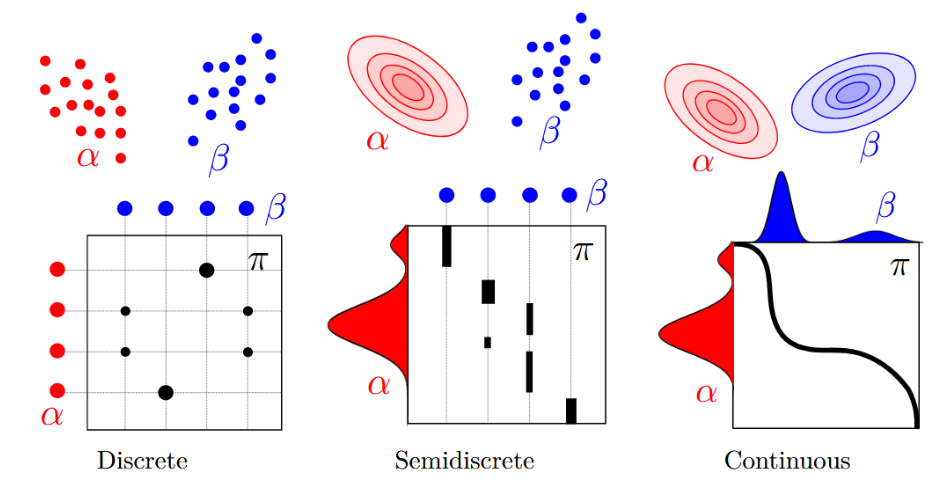
\includegraphics[scale=0.2]{Kantorovich-relaxation.png}
    \caption{\label{fig:label} }
  \end{figure}
\end{frame}

\begin{frame}
  \frametitle{}
  \begin{block}{Example (as before)}
    $X=(x_1, \dots, x_m)$ and $Y=(y_1, \dots, y_n)$ and
    $\mu= \frac{1}{m}(\delta_{x_1}+ \cdots + \delta_{x_m})$ and $\nu= \frac{1}{n}(\delta_{y_1}+ \cdots + \delta_{y_m})$
  \end{block}
  The problem reduces to
  \begin{equation}
    \min_{\gamma} \sum_{i,j} C_{i,j} \gamma_{i,j},
  \end{equation}
  where again $C_{i,j}$ is the cost of moving mass from $x_i$ to $y_j$
  Then the space of probability measures on $X\times Y$ is just the set of matrices ${[\gamma_{i,j}]}_{i=1,\dots,m, j=1,\dots,n}$
  such that
  \begin{equation}
    \sum_{i=1}^{m} \gamma_{i,j} = \frac{1}{n} \quad \text{and} \quad \sum_{j=1}^{n} \gamma_{i,j} = \frac{1}{m}
  \end{equation}
  called \textbf{bistochastic matrices}.
\end{frame}

\begin{frame}
  \frametitle{Doubly stochastic matrices and the Birkhoff polytope}
  If $m=n$, then
  \begin{equation}
    \sum_{i=1}^{m} \gamma_{i,j} = \frac{1}{n} = \sum_{j=1}^{n} \gamma_{i,j}
  \end{equation}
  which called \textbf{bistochastic matrices} (scaled by \frac{1}{n}).\\
  The set of all such matrices is called the \textbf{Birkhoff polytope}.

  \onslide<2->{%
    \begin{block}{Vertices of the Birkhoff polytope}
      Are given by the permutation matrices.
    \end{block}
  }
  \onslide<3->{%
    By linearity
  \begin{equation}
    \begin{aligned}
    &\min_{\gamma \in \Pi} \sum_{i,j} C_{i,j} \gamma_{i,j}\\
    &= \frac{1}{n}\min_{\gamma \in Perm}\sum_{i,j} C_{i,j} \gamma_{i,j}
    &= \frac{1}{n} \min_{\sigma}\sum_{i,j} C_{i,\sigma(i)}
    \end{aligned}
  \end{equation}
  }
\end{frame}

\begin{frame}
  \frametitle{}
  \begin{block}{Example (with non-uniform distribution)}
    Now $\mu = p = (p_1, \dots, p_m)$ and $\nu = q = (q_1, \dots, q_n)$
  \end{block}
  \begin{equation}
    \begin{aligned}
      K(\mu, \nu) &= \min_\gamma \sum_{}^{} C_{i,j} \gamma_{i,j} \\
      s.t. & \begin{cases}
        \sum_{i}^{} \gamma_{i,j} = q_j \\
        \sum_{j}^{} \gamma_{i,j} = p_i \\
        \gamma_{i,j} \ge 0
      \end{cases}
    \end{aligned}
  \end{equation}
  Linear optimization problem.
\end{frame}

% Write here about wasserstein distance?
% \section{Wasserstein distance}%
% \label{sec:}


\end{document}
